\chapter{Fundamentação Teórica}\label{cap:fundamentacao}

Este capítulo reúne os conceitos necessários para situar a comparação entre
as arquiteturas de aquisição investigadas neste trabalho. Parte-se do
teorema da amostragem e das fontes de erro temporal que afetam um sistema de
aquisição embarcado (Seções~\ref{sec:determinismo} a~\ref{sec:interrupt}),
segue-se para os mecanismos de hardware do RP2350 empregados na abordagem
dedicada, isto é, \ac{PIO}, \ac{DMA} e o \ac{RLE} (Seção~\ref{sec:hardware}), e
para a discussão sobre a ausência de \ac{RTOS} no projeto
(Seção~\ref{sec:baremetal-vs-rtos}). Por fim, apresenta-se o ecossistema
Sigrok/PulseView e o protocolo sigrok-pico (Seção~\ref{sec:sigrok-pico}),
sobre o qual ambos os firmwares comparados são construídos, e revisam-se os
trabalhos relacionados que motivam a comparação proposta.

\section{Aquisição de sinais digitais e o teorema da amostragem}

A transformação de um sinal contínuo no tempo em uma sequência digital é regida
pelo teorema da amostragem de Nyquist--Shannon, que estabelece que um sinal
deve ser amostrado a uma taxa pelo menos superior ao dobro de sua maior
componente de frequência para que possa ser reconstruído sem ambiguidade
\cite{nyquist1928,shannon1949,proakis1996}. Quando essa condição é violada,
ocorre o fenômeno de \emph{aliasing}: componentes acima da metade da taxa de
amostragem aparecem mascaradas como frequências mais baixas nos dados
adquiridos, corrompendo permanentemente a informação capturada 
\cite{smith1999}. Como ilustra a Figura~\ref{fig:aliasing}, quando a taxa de
amostragem é insuficiente ($f_s < 2f_{sinal}$), os pontos amostrados (em
destaque) passam a descrever uma senoide de frequência muito menor que a do
sinal original, produzindo um alias que substitui irreversivelmente a
informação real.

\begin{figure}[H]
  \centering
  \caption{Efeito de \emph{aliasing} na amostragem de uma senoide.}
  \label{fig:aliasing}
  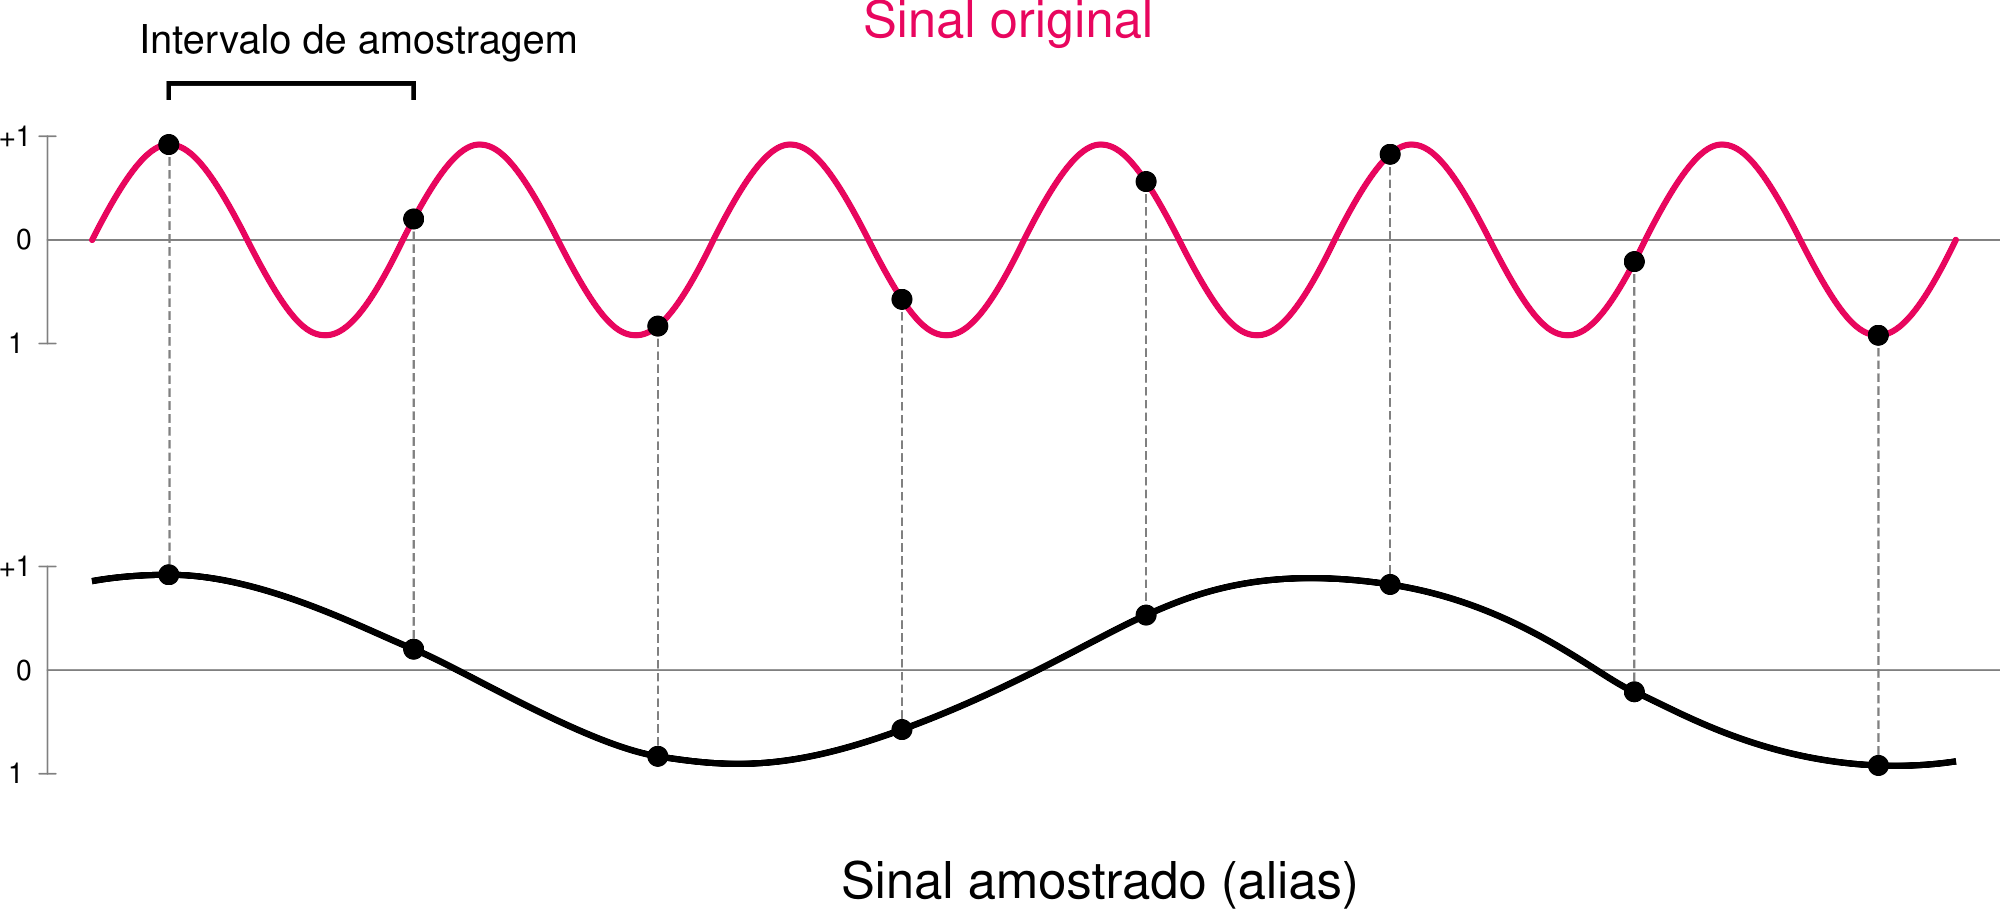
\includegraphics[width=0.7\linewidth]{Cap02/img/aliasing_wikimedia.png}
  \fonte{adaptado de \citeonline{krol_aliasing}, licença CC0.}
  \nota{sinal original em rosa; sinal percebido a partir das amostras em preto.}
\end{figure}

Para um analisador lógico, o requisito prático é ainda mais estrito que o
limite teórico. A reconstrução fiel de uma forma de onda digital, incluindo
a posição temporal das bordas, a largura de pulsos estreitos e \emph{glitches}, exige tipicamente uma taxa de amostragem de quatro a dez vezes a frequência
fundamental do sinal observado e, mais importante, exige que o intervalo entre
amostras seja constante: qualquer variação no período de amostragem se
traduz diretamente em erro na posição medida das bordas
\cite{smith1999,gis2021}.

\section{Determinismo temporal em sistemas embarcados}\label{sec:determinismo}

Em sistemas de aquisição, o termo determinismo designa a propriedade
de um evento de software ou hardware ocorrer em instantes previsíveis,
ciclo a ciclo. Três grandezas caracterizam o desvio desse ideal
\cite{lee2017,gis2021,alonso2024}:

\begin{itemize}
  \item \textbf{Latência}: o atraso entre um evento físico (por exemplo, uma borda de sinal) e a reação do sistema (o registro da amostra ou o início da captura); na Figura~\ref{fig:latencia-jitter-vazao}, corresponde ao deslocamento entre o evento esperado e a resposta real;
  \item \textbf{\emph{Jitter}}: a variação estatística dessa latência ou, no caso da amostragem periódica, a variação do intervalo entre amostras consecutivas em torno do período nominal; na Figura~\ref{fig:latencia-jitter-vazao}, é a diferença de latência de um ciclo para outro;
  \item \textbf{Vazão} (\emph{throughput}): a quantidade de dados que o sistema sustenta por unidade de tempo sem perdas; na Figura~\ref{fig:latencia-jitter-vazao}, é a taxa de amostras sustentada no intervalo observado.
\end{itemize}

\begin{figure}[H]
  \centering
  \caption{Latência, \emph{jitter} e vazão.}
  \label{fig:latencia-jitter-vazao}
  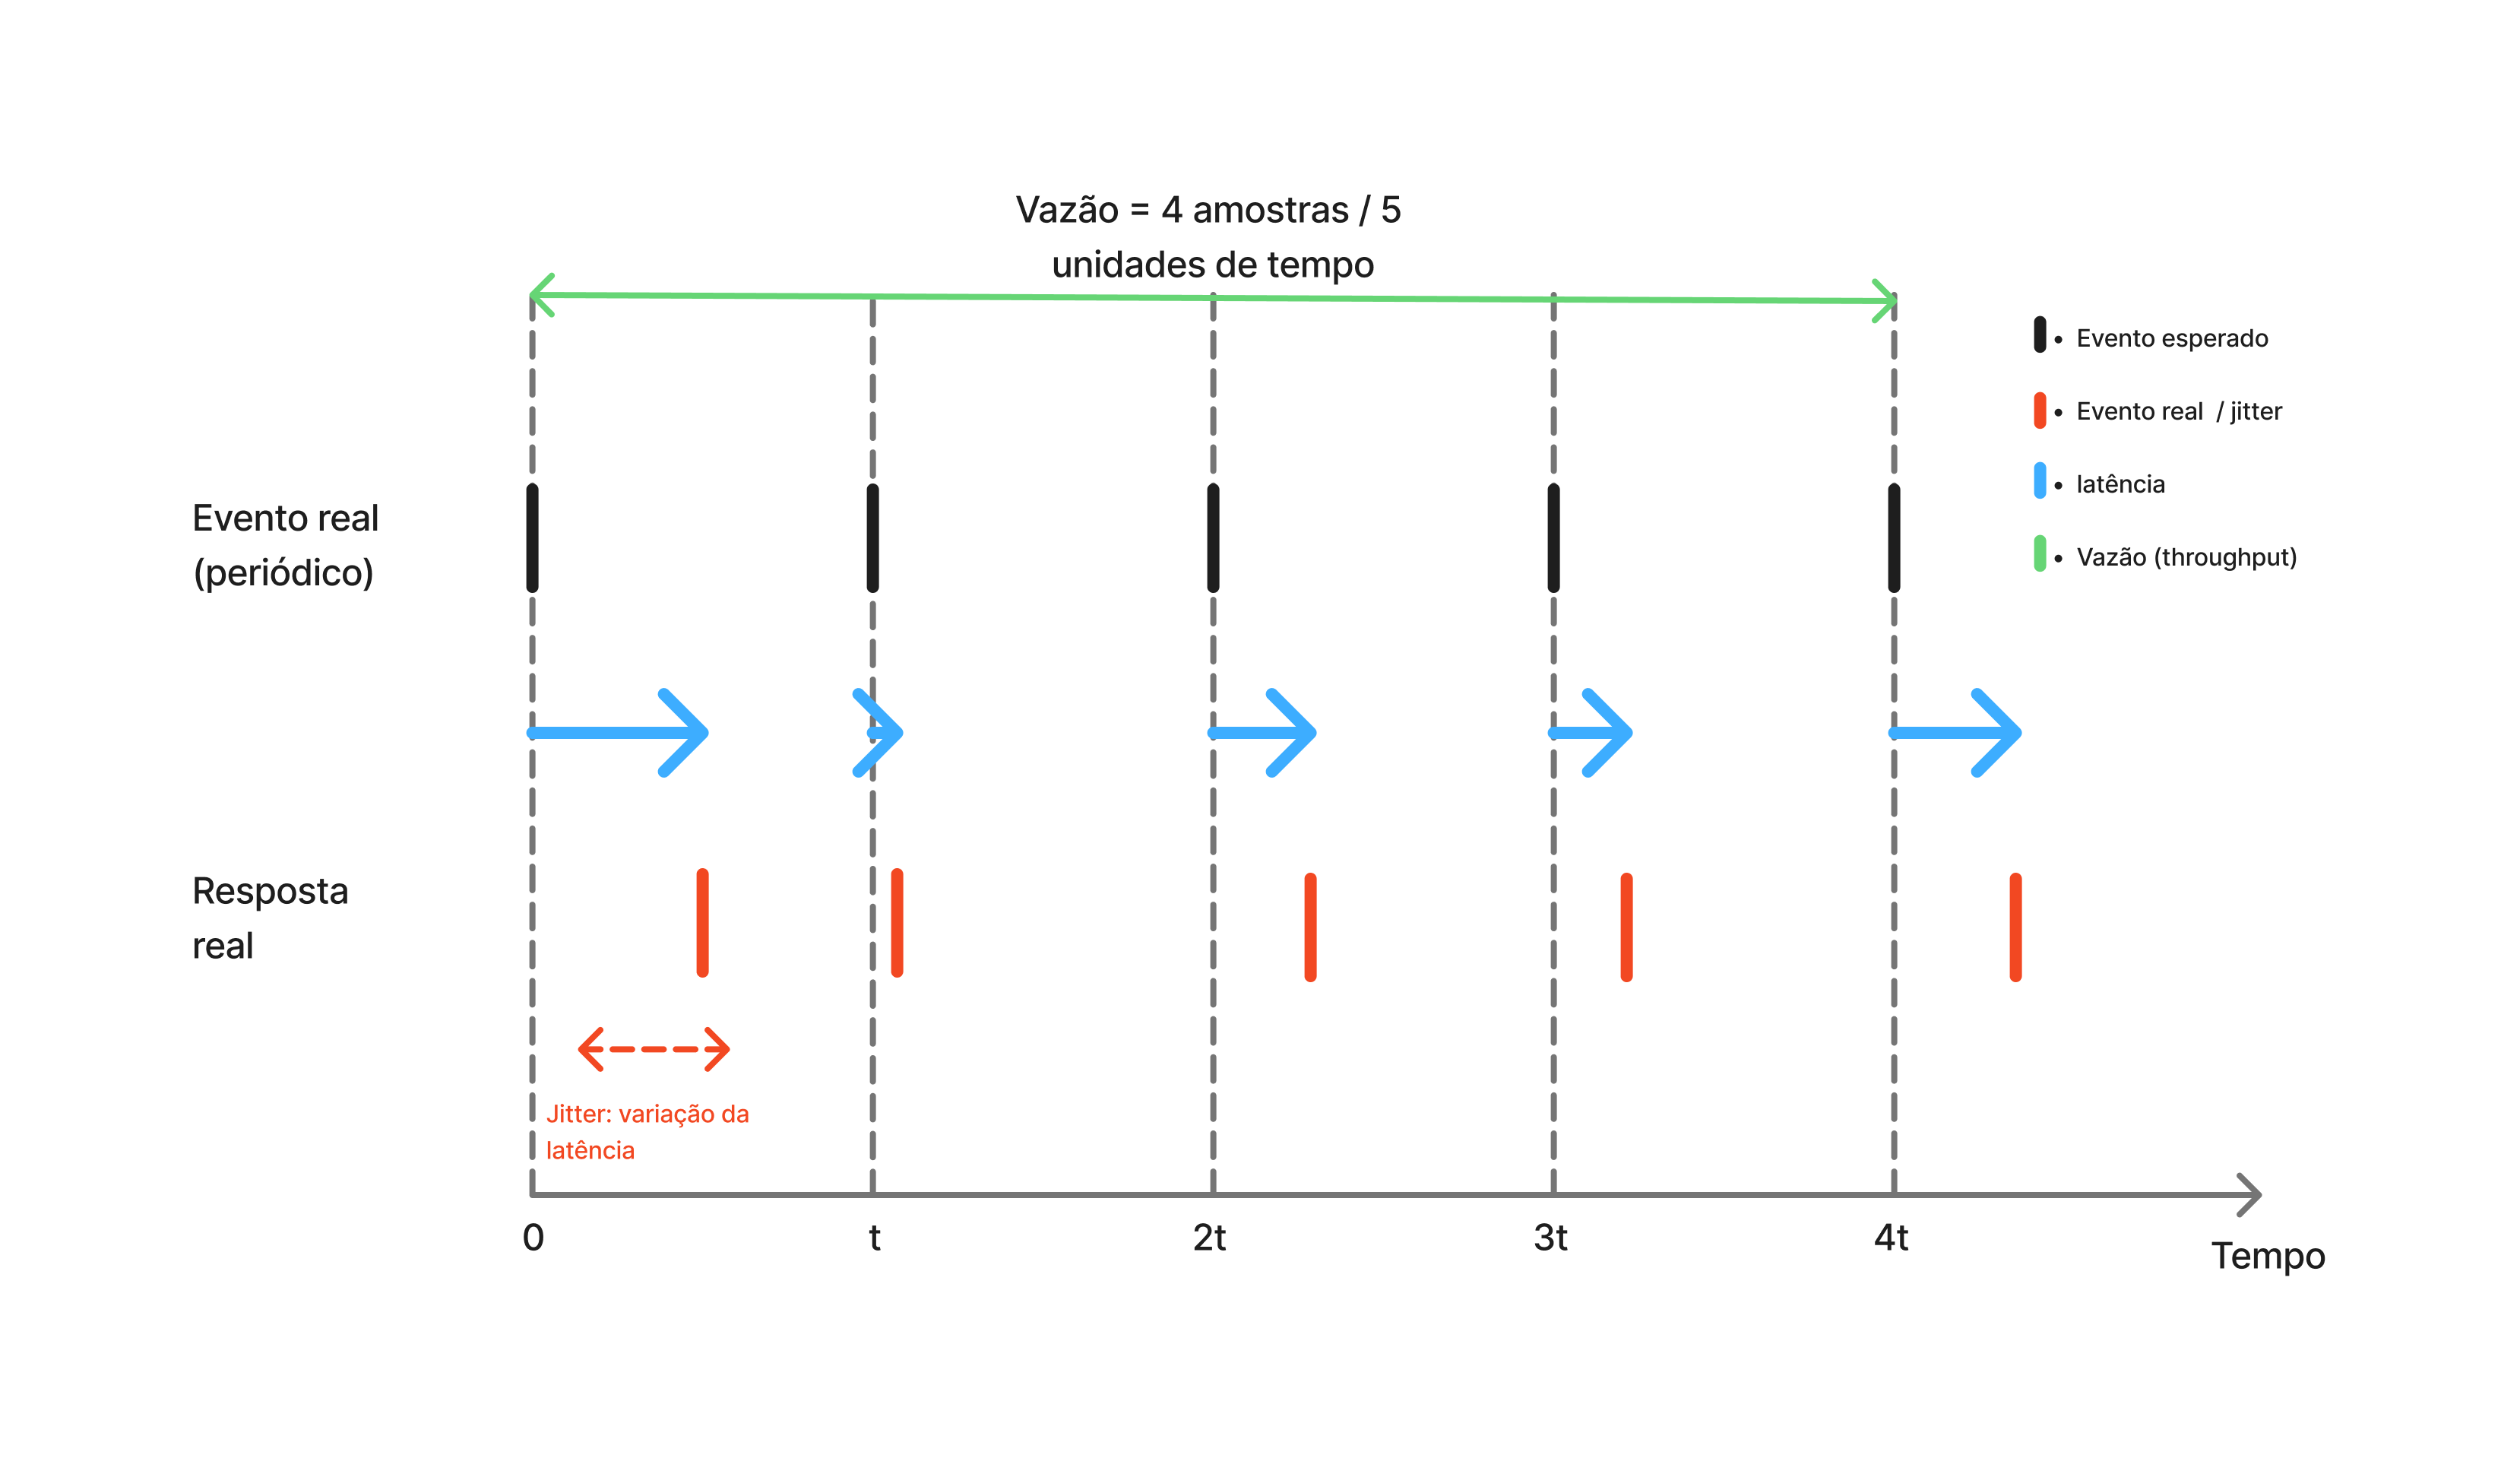
\includegraphics[width=0.85\linewidth]{Cap02/img/latencia_jitter_vazao.png}
  \fonte{Autoria própria.}
\end{figure}

Em um microcontrolador executando o padrão \ac{GPIO} com \ac{CPU}, captura de
sinais digitais por \emph{polling} ou interrupção, as causas vistas na Figura~\ref{fig:latencia-jitter-vazao}
tornam-se observáveis na Figura~\ref{fig:fontes-jitter-gpio-cpu}: diversas
fontes degradam o determinismo \cite{lee2017,ungurean2020,alonso2024}:

\begin{enumerate}
  \item \textbf{Latência de interrupção}: entre a ativação de uma \ac{IRQ} e a primeira instrução útil da \ac{ISR} decorre, já no melhor caso, da ordem de uma dezena de ciclos (tipicamente 12 no Cortex-M33, para salvamento de contexto, resolução de prioridade e busca do vetor), e esse número cresce e varia conforme a instrução em execução no momento e o estado do \emph{pipeline} \cite{arm2021};
  \item \textbf{Concorrência de interrupções}: \acp{ISR} de maior prioridade (por exemplo, da pilha \ac{USB}) atrasam a \ac{ISR} ou o laço de aquisição de forma imprevisível;
  \item \textbf{Troca de contexto (\acs{RTOS})}: em sistemas com escalonador, o \emph{tick} periódico e as trocas de tarefa consomem ciclos e adiam o atendimento de eventos; como o firmware de referência deste trabalho é \emph{bare-metal}, construído sobre o Raspberry Pi Pico \ac{SDK} e sem \ac{RTOS} (Seção~\ref{sec:baremetal-vs-rtos}), essa fonte específica não se aplica à implementação avaliada, mas é listada aqui por completude, já que caracteriza o padrão \ac{GPIO} com \ac{CPU} em geral;
  \item \textbf{Hierarquia de memória}: em chips que executam código diretamente da flash externa, em modo de \ac{XIP}, uma falha de cache impõe esperas de dezenas de ciclos no meio de um laço que se pretendia de tempo constante;
  \item \textbf{Arbitragem de barramento}: acessos simultâneos de \ac{CPU}, \ac{DMA} e periféricos à mesma \ac{SRAM} podem inserir ciclos de espera.
\end{enumerate}


A Figura~\ref{fig:fontes-jitter-gpio-cpu} resume essa cadeia de fontes, do evento físico
ao registro final da amostra. Para a amostragem periódica, o efeito agregado dessas fontes é o \emph{jitter}
de amostragem, que corrompe a base de tempo da aquisição: uma amostra tomada
tarde demais desloca a borda medida, e o erro não é recuperável por
pós-processamento. É por essa razão que plataformas de aquisição de alta
velocidade tradicionalmente recorrem a hardware dedicado, \acp{ASIC} ou \acp{FPGA}, em
que a amostragem é síncrona a um clock físico e imune ao estado do software
\cite{dai2017,gis2021}. O custo dessas soluções, entretanto, é justamente a
barreira que a instrumentação baseada em microcontrolador busca contornar,
conforme demonstram \citeonline{hercog2014} e \citeonline{romanov2021}.

\begin{figure}[htbp]
  \centering
  \caption{Fontes de não determinismo no padrão GPIO+CPU.}
  \label{fig:fontes-jitter-gpio-cpu}
  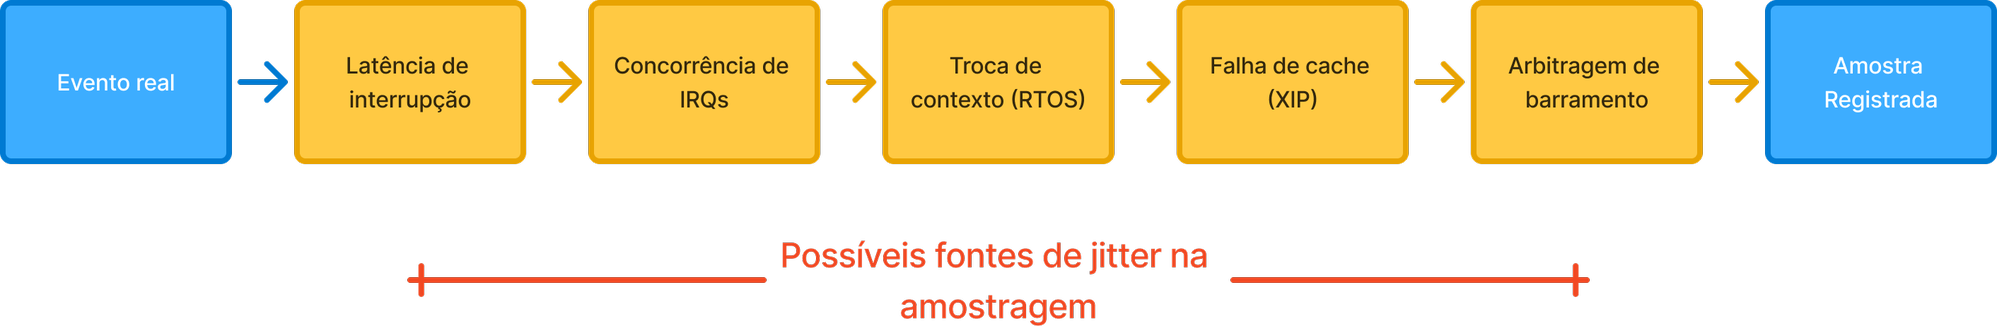
\includegraphics[width=0.9\linewidth]{Cap02/img/fontes_jitter_gpio_cpu.png}
  \fonte{Autoria própria.}
\end{figure}

\section{Aquisição por software}

\subsection{Aquisição com \emph{polling}}\label{sec:polling}

A abordagem mais direta para capturar sinais digitais em um \ac{MCU} é ler
periodicamente o registrador de entrada dos \acp{GPIO} com a própria \ac{CPU}, técnica
conhecida como \emph{polling} \cite{patterson2017}. Um laço mínimo de
amostragem executa, a cada iteração: a leitura do registrador de entrada, o
armazenamento do valor em um buffer, o avanço do ponteiro e o desvio
condicional de volta ao início. A taxa de amostragem máxima é, portanto,
limitada por:

\begin{equation}\label{eq:fsmax}
  f_{s,\max} = \frac{f_{clk}}{C_{iter}}
\end{equation}

\noindent em que $f_{clk}$ é a frequência da \ac{CPU} e $C_{iter}$ o número de ciclos por iteração do laço. Mesmo em um laço cuidadosamente otimizado em C ou assembly, da ordem de 4 a 8 ciclos por iteração em um Cortex-M33 com buffer em \ac{SRAM}, um clock de \ac{CPU} de 150\,MHz limita a amostragem a poucas dezenas de mega-amostras por segundo \emph{no melhor caso}, e qualquer instrução adicional (verificação de parada, controle de taxa, empacotamento) reduz esse teto proporcionalmente \cite{patterson2017,rpi2024ds}.

Mais grave que o teto de vazão é a instabilidade do período: para
amostrar a uma taxa \emph{programável} (e não simplesmente ``o mais rápido
possível''), o laço precisa calibrar sua duração com instruções de espera ou
comparação contra um \emph{timer}, e cada evento assíncrono (interrupção da
pilha \ac{USB}, falha de cache \ac{XIP}, acesso concorrente de \ac{DMA} à \ac{SRAM}) alonga
iterações individuais, produzindo \emph{jitter}. Desabilitar as interrupções
elimina parte do problema, mas impede o atendimento da comunicação com o \emph{host}
durante a captura, o que inviabiliza a captura contínua com transmissão
simultânea (\emph{streaming}).

\subsection{Aquisição com \emph{interrupção}}\label{sec:interrupt}

A alternativa por interrupção, configurar uma \ac{IRQ} de borda no \ac{GPIO} e
registrar amostras na \ac{ISR}, desloca o problema sem resolvê-lo: em frequências
altas, transições rápidas geram interrupções em cadência superior à capacidade
de atendimento da \ac{CPU}, sobrecarregando-a e causando perda de amostras e
corrupção de dados, fenômeno descrito na literatura de sistemas como
\emph{receive livelock}, em que a vazão útil colapsa a zero quando a taxa de
eventos excede a capacidade de atendimento da \ac{CPU}
\cite{mogul1997,regehr2005,souza2020}. Por isso, a aquisição por interrupção é
adequada apenas a sinais esparsos e lentos e não foi incluída na comparação
experimental deste trabalho, que adota o \emph{polling} como representante da
abordagem por software.

Uma mitigação relevante em \acp{MCU} de dois núcleos é \textbf{dedicar um núcleo
  inteiro ao laço de amostragem}, deixando o outro responsável pela comunicação.
Essa variante elimina a disputa direta entre amostragem e \ac{USB}, mas não elimina
o teto de vazão do laço nem as interferências de barramento e de memória e
ocupa integralmente um recurso computacional que, na arquitetura por hardware,
permanece livre. Essa variante é descrita na Seção~\ref{sec:firmware-b}, mas
não foi avaliada experimentalmente, ficando como trabalho futuro
(Seção~\ref{sec:trabalhos-futuros}).

\section{Aquisição por hardware: RP2350B}\label{sec:hardware}


\subsection{O microcontrolador RP2350}

O RP2350, da Raspberry Pi, é um microcontrolador de dois núcleos, ARM
Cortex-M33 ou RISC-V Hazard3, selecionáveis na inicialização, operando
tipicamente a 150\,MHz, com 520\,KB de \ac{SRAM} interna (512\,KB principais, distribuídos em oito
bancos, e dois bancos auxiliares de 4\,KB) e sem
memória flash interna: o código reside em uma flash \ac{QSPI} externa e é executado
via \ac{XIP} com cache \cite{rpi2024ds}. O chip dispõe de um
\ac{SIO}, que permite à \ac{CPU} ler o estado de todos os \acp{GPIO} em uma única
instrução, recurso central para a variante por software deste trabalho, além de
um conversor analógico-digital de 12 bits e dos subsistemas \ac{PIO} e \ac{DMA} descritos
a seguir. A variante RP2350B, utilizada na plataforma deste trabalho, expõe 48
\acp{GPIO} \cite{rpi2024ds}. A Figura~\ref{fig:rp2350-bus} mostra o
\emph{crossbar} \ac{AHB}5 que interliga esses recursos: os dois núcleos, o \ac{DMA} e os
periféricos (incluindo os três blocos \ac{PIO}) disputam as portas de \ac{SRAM}, \ac{XIP} e
\ac{APB}, e é justamente nesse ponto de disputa que se origina a arbitragem de
barramento citada como fonte de \emph{jitter} na Seção~\ref{sec:determinismo}.

\begin{figure}[htbp]
  \centering
  \caption{\emph{Crossbar} AHB5 do RP2350.}
  \label{fig:rp2350-bus}
  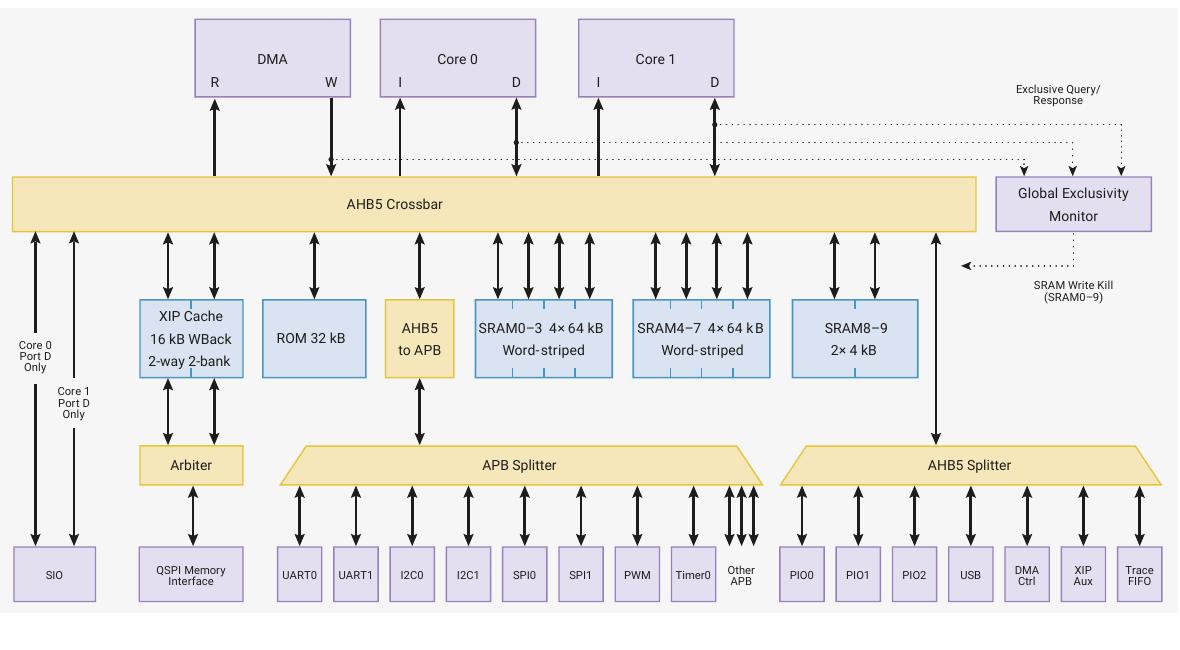
\includegraphics[width=0.7\linewidth]{Cap02/img/rp2350_bus_fabric.png}
  \fonte{\citeonline{rpi2024ds}.}
\end{figure}

\subsection{O subsistema PIO}\label{sec:pio}

O \ac{PIO} (\emph{Programmable Input/Output}) é o diferencial arquitetural da
família RP2 para aplicações de aquisição. Trata-se de blocos independentes
contendo, cada um, quatro \acp{SM} de hardware que executam um
conjunto de instruções próprio, minimalista e determinístico, em que cada
instrução executa em exatamente um ciclo do clock da máquina de estados
\cite{rpi2024ds}. O RP2350 integra três blocos \ac{PIO}, totalizando doze máquinas
de estados. A Figura~\ref{fig:pio-block} detalha a organização interna de um
desses blocos: as quatro máquinas de estado independentes compartilham a
memória de instruções e trocam dados com o barramento do sistema por meio de
\acp{FIFO} de hardware, sem intervenção da \ac{CPU}.

\begin{figure}[H]
  \centering
  \caption{Diagrama de blocos do PIO.}
  \label{fig:pio-block}
  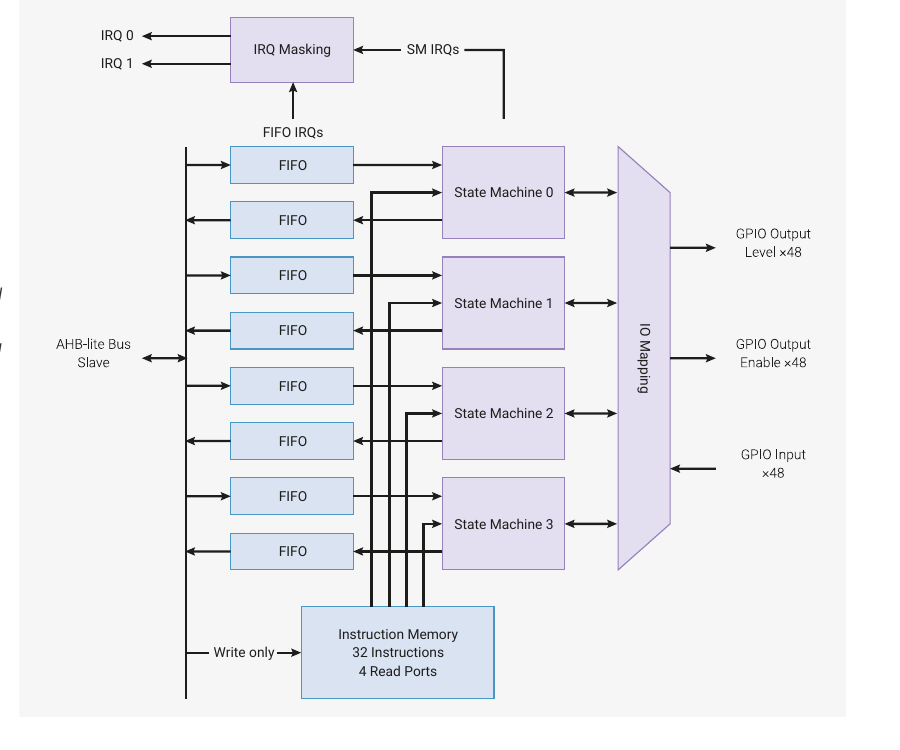
\includegraphics[width=0.75\linewidth]{Cap02/img/rp2350_pio_block_diagram.png}
  \fonte{\citeonline{rpi2024ds}.}
\end{figure}

Diferentemente de um laço de software na \ac{CPU}, uma máquina de estados \ac{PIO} pode
amostrar múltiplos pinos simultaneamente e empurrar os dados para um buffer
\ac{FIFO} de hardware, sem sofrer latência de interrupção, sobrecarga de troca de
contexto ou \emph{jitter} de execução, pois opera de forma totalmente
independente dos núcleos principais \cite{rpi2024ds,weber2025,mehr2025}. O
período de amostragem é definido por um divisor de clock fracionário próprio de
cada máquina de estados:

\begin{equation}\label{eq:clkdiv}
  \text{clkdiv} = \frac{f_{sys}}{f_{sample}}
\end{equation}

\noindent em que o divisor é representado em ponto fixo, com parte fracionária
de oito bits \cite{rpi2024ds}. Para divisores inteiros, o período de amostragem
é rigorosamente fixo em ciclos do clock do sistema. Para divisores
fracionários, a máquina de estados aproxima a taxa média alternando entre dois
períodos inteiros adjacentes, o que introduz um \emph{jitter} determinístico de
até um ciclo de $f_{sys}$, cerca de 6,7\,ns a 150\,MHz, no instante de
cada amostra \cite{rpi2024ds}. Esse limite é duas ordens de grandeza menor que
o período de amostragem nas taxas aqui investigadas e, ao contrário do laço de
\emph{polling} (Seção~\ref{sec:polling}), não depende do caminho de execução da
\ac{CPU} nem da latência de interrupção. Essa previsibilidade decorre do próprio
conjunto de instruções do \ac{PIO}, resumido a seguir.

\subsubsection{O conjunto de instruções do PIO}\label{sec:pio-isa}

O \ac{PIO} executa um conjunto reduzido de nove instruções, todas com duração fixa
de um ciclo de clock da máquina de estados (exceto quando programadas para
aguardar explicitamente), o que torna o tempo de execução de qualquer programa
previsível em tempo de compilação \cite{rpi2024ds}. Para a aquisição de
sinais digitais, duas instruções são centrais:

\begin{itemize}
  \item \texttt{in pins, N}: desloca o estado instantâneo de N pinos de
  entrada para o registrador de deslocamento e, quando este se enche, empurra
  automaticamente seu conteúdo para o \ac{FIFO} de recepção. Um programa de captura
  mínimo é essa única instrução em laço, produzindo uma amostra de N pinos por
  ciclo com comportamento \emph{cycle-accurate} que espelha o determinismo de
  um \ac{FPGA} a uma fração do custo \cite{rpi2024ds};
  \item \texttt{jmp pin}: desvia o fluxo do programa conforme o estado
  instantâneo de um \ac{GPIO} designado, sem consumir ciclos adicionais de
  amostragem, permitindo implementar disparo (\emph{trigger}) por borda ou por
  nível inteiramente em hardware \cite{rpi2024ds,starkey2024}.
\end{itemize}

\subsection{O subsistema DMA}

A captura contínua em alta taxa gera um fluxo de dados que rapidamente excede a
capacidade dos \acp{FIFO} internos do \ac{PIO} (quatro palavras por máquina de estados;
oito quando os \acp{FIFO} de transmissão e recepção são concatenados). Para evitar
transbordamento e perda de dados, emprega-se o controlador de \ac{DMA}: um
subsistema de hardware especializado em transferir dados entre periféricos e
memória sem intervenção da \ac{CPU} \cite{patterson2017,rpi2024ds}. No RP2350, cada
canal de \ac{DMA} pode ser ritmado pelo \ac{DREQ} do
periférico, de modo que a transferência avança automaticamente quando há dados
novos e estaciona quando o \ac{FIFO} esvazia. A Figura~\ref{fig:dma-architecture}
detalha essa arquitetura interna: gerentes de leitura e escrita independentes
movimentam dados entre memória e periféricos através de \acp{FIFO} de endereço e de
transferência, operando sobre o barramento do sistema sob supervisão apenas
dos registradores de controle e status.

\begin{figure}[H]
  \centering
  \caption{Arquitetura do controlador de DMA do RP2350.}
  \label{fig:dma-architecture}
  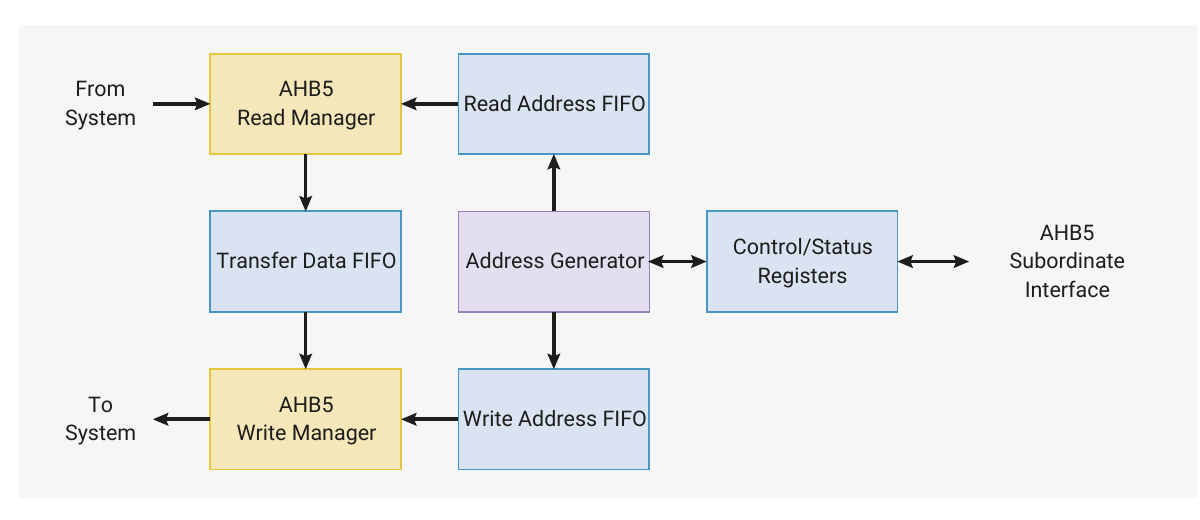
\includegraphics[width=0.85\linewidth]{Cap02/img/rp2350_dma_architecture.png}
  \fonte{\citeonline{rpi2024ds}.}
\end{figure}

Dois recursos são particularmente relevantes para aquisição contínua: o
\textbf{encadeamento de canais} e a operação em \textbf{\emph{ping-pong}}, em
que dois canais (ou dois blocos de descritores) se alternam entre duas metades
de um buffer enquanto o \ac{DMA} preenche uma metade, a \ac{CPU} (ou um segundo canal)
escoa a outra, com uma interrupção sinalizando cada troca de metade. Essa
técnica desacopla completamente a produção de amostras
(\ac{PIO}$\rightarrow$\ac{DMA}$\rightarrow$\ac{SRAM}) do consumo (\ac{SRAM}$\rightarrow$\ac{USB}),
permitindo \emph{streaming} sem lacunas \cite{rpi2024ds}.

Essa arquitetura reduz drasticamente a cadeia de fontes de \emph{jitter}
identificada para o padrão \ac{GPIO} com \ac{CPU} (Figura~\ref{fig:fontes-jitter-gpio-cpu}).
Como ilustra a Figura~\ref{fig:fontes-jitter-pio-dma}, o trecho crítico,
máquina de estados do \ac{PIO} $\rightarrow$ \ac{FIFO} de hardware $\rightarrow$
transferência via \ac{DMA} para a \ac{SRAM}, é inteiramente síncrono ao clock da
máquina de estados e ocorre sem intervenção da \ac{CPU}, portanto livre das fontes
de \emph{jitter} de software. O efeito de um
eventual atraso nesse trecho também muda de natureza: como a amostra já foi
capturada pelo \ac{PIO} no instante correto, um atraso na troca de \emph{buffer}
não desloca o instante de nenhuma amostra, e o risco passa a ser
\emph{overflow} da \ac{FIFO} (perda de amostras), não \emph{jitter} de
temporização.

\begin{figure}[H]
  \centering
  \caption{Fontes de não determinismo no padrão PIO+DMA.}
  \label{fig:fontes-jitter-pio-dma}
  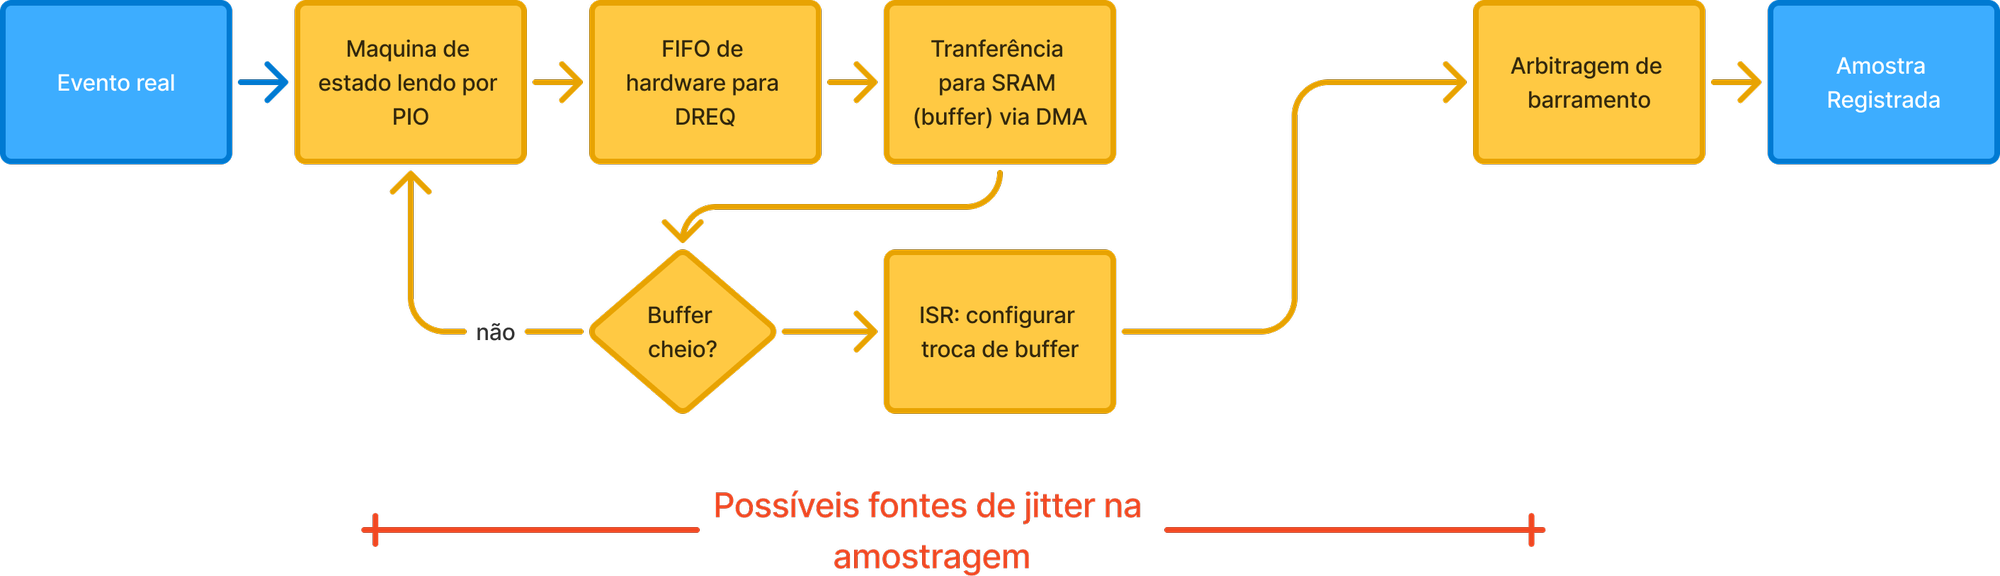
\includegraphics[width=0.95\linewidth]{Cap02/img/fontes_jitter_pio_dma.png}
  \fonte{Autoria própria.}
\end{figure}

A delegação da movimentação de dados ao \ac{DMA} é uma estratégia bastante conhecida
para maximizar a eficiência de sistemas embarcados com recursos restritos,
já que libera a \ac{CPU} de copiar cada dado entre periférico e memória
\cite{rpi2024ds}.

\subsection{Codificação (RLE)}

Depois que o \ac{DMA} deposita as amostras na \ac{SRAM}, a \ac{CPU} volta a entrar no
caminho de dados, mas fora do trecho crítico de captura: sua tarefa é
comprimir o \emph{buffer} por \acf{RLE} antes do envio via \ac{USB}, reduzindo a banda exigida
quando as linhas permanecem estáveis por várias amostras consecutivas. Em
vez de transmitir cada amostra, o \ac{RLE} transmite o valor e o número de
repetições consecutivas desse valor: uma linha estável por milhares de
amostras ocupa poucos \emph{bytes}. O ganho, porém, depende do sinal: um
sinal com transições a quase toda amostra praticamente não se compacta, de
modo que a banda exigida do \ac{USB} passa a depender do padrão capturado, efeito
que condiciona o desenho experimental (Seção~\ref{sec:bancada}). O formato
exato dos pares valor--repetição é definido pelo protocolo sigrok-pico
(Seção~\ref{sec:sigrok-pico}) e resumido na Seção~\ref{sec:firmware-a}.

\section{\emph{Bare-metal} \emph{versus} RTOS}\label{sec:baremetal-vs-rtos}

Um \acf{RTOS} introduz um escalonador cujo
\emph{tick} periódico realiza trocas de contexto entre tarefas, atribuindo
fatias de tempo e prioridades a cada uma delas. Esse mecanismo resolve um
problema de concorrência entre tarefas de propósito geral, mas não elimina o
não determinismo inerente ao restante do sistema: a latência de
escalonamento soma-se, e não substitui, as demais fontes de \emph{jitter}
discutidas na Seção~\ref{sec:determinismo} (latência de interrupção,
hierarquia de memória, arbitragem de barramento). Para uma tarefa em que a
temporização deve ser exata em ciclos e livre de \emph{jitter}, como a
amostragem de um analisador lógico, a sincronização de software oferecida por
um \ac{RTOS} não traz benefício sempre que a temporização crítica puder ser
garantida diretamente pelo hardware, e não pelo software
\cite{ungurean2020,hui2023}.

\section{O ecossistema Sigrok/PulseView e o protocolo sigrok-pico}\label{sec:sigrok-pico}

O Sigrok é uma suíte de software livre, portável e multiplataforma para
aquisição e análise de sinais, que abstrai dezenas de instrumentos por meio da
biblioteca \texttt{libsigrok}; o PulseView é seu \emph{front-end} gráfico, com
biblioteca de mais de duzentos decodificadores de protocolo: \ac{I2C}, \ac{SPI}, \ac{UART},
\ac{CAN}, RS-232, RS-485, entre outros, aplicáveis diretamente sobre os dados
capturados \cite{sigrok2026}. A Figura~\ref{fig:pulseview} mostra essa
decodificação em funcionamento: a faixa superior exibe um decodificador de
protocolo sobrepondo os bytes reconhecidos às formas de onda digitais brutas
exibidas logo abaixo.

\begin{figure}[htbp]
  \centering
  \caption{Captura decodificada no PulseView.}
  \label{fig:pulseview}
  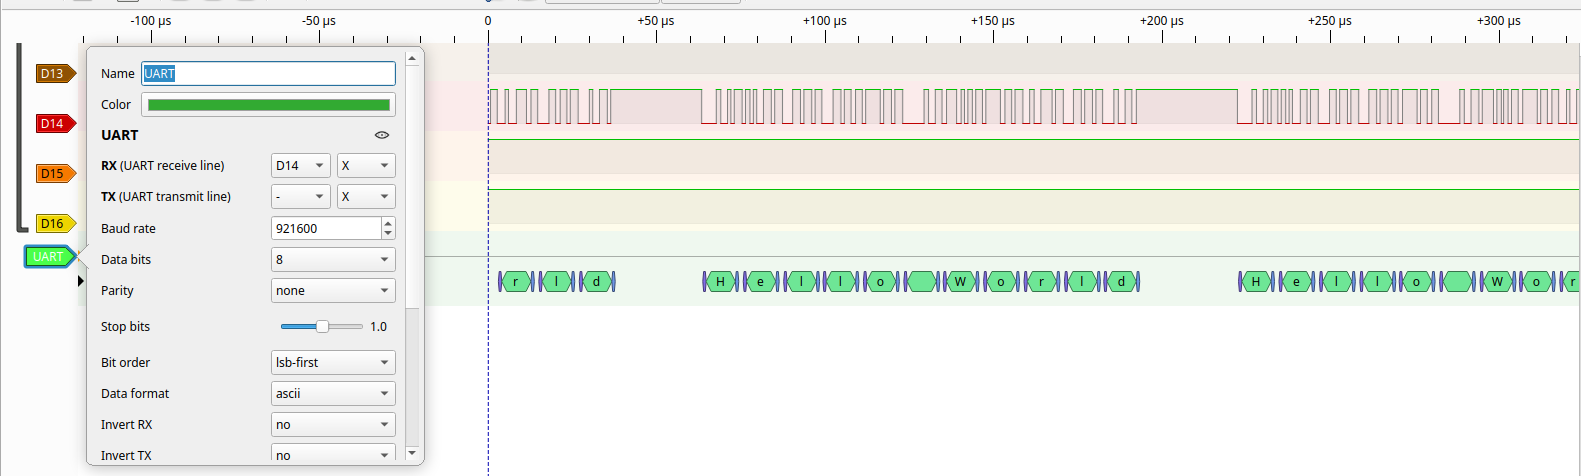
\includegraphics[width=0.95\linewidth]{Cap02/img/pulseview_screenshot.png}
  \fonte{adaptado de \citeonline{sigrok2026} (licença GNU GPL).}
\end{figure}

A adoção desse ecossistema como interface de
\emph{host} elimina os custos de licenciamento associados a softwares proprietários de
análise e transfere ao \emph{host} todo o processamento pesado (decodificação,
medição, exportação), exigindo do firmware apenas a conformidade com a
especificação do protocolo serial \textbf{sigrok-pico} \cite{picocoder2023}:
um protocolo textual simples sobre \ac{USB} \ac{CDC} explicitado no Quadro~\ref{qua:comandos}.

\section{Trabalhos relacionados}

O uso de microcontroladores da família RP2 como analisadores lógicos de baixo
custo tem precedentes na comunidade de software livre. O projeto
\textbf{sigrok-pico} \cite{picocoder2023}, origem do protocolo adotado,
implementa captura de até 21 canais digitais via \ac{PIO} com transferência por \ac{DMA}
no RP2040, com \emph{fork} posterior para o RP2350, e outros projetos
comunitários seguem a mesma linha. Esses projetos demonstram a viabilidade
da abordagem do \ac{PIO} associado ao \ac{DMA}, mas nenhum deles quantifica o ganho
sobre a alternativa por software: a escolha pelo \ac{PIO} é assumida como
evidente e não é medida.

Na literatura acadêmica, os trabalhos consultados cobrem partes da questão,
mas não a comparação em si. \citeonline{hercog2014} e \citeonline{romanov2021}
mostram que instrumentação de aquisição e análise lógica baseada em
microcontrolador é viável e reprodutível, sem contrapor arquiteturas de
captura. \citeonline{gis2021} e \citeonline{ungurean2020} caracterizam
experimentalmente o \emph{jitter} e o não determinismo da execução em
microcontroladores, fornecendo o arcabouço para as fontes discutidas na
Seção~\ref{sec:determinismo}, mas não em um instrumento de aquisição.
\citeonline{regehr2005} e \citeonline{mogul1997} descrevem o mecanismo pelo qual
sistemas dirigidos a interrupção saturam sob alta taxa de eventos
(Seção~\ref{sec:interrupt}). Por fim, \citeonline{weber2025}, \citeonline{starkey2024}
e \citeonline{mehr2025} empregam o \ac{PIO} e o \ac{DMA} do RP2040/RP2350 como periféricos
de temporização determinística em instrumentação científica, adotando o
hardware dedicado sem medi-lo contra a leitura por software. Nenhum desses
trabalhos mede, na mesma plataforma e sob as mesmas condições, taxa
sustentada, \emph{jitter}, perda de amostras e ocupação de \ac{CPU} das duas
arquiteturas, que é a comparação conduzida neste trabalho
(Capítulo~\ref{cap:metodologia}).
O Quadro~\ref{qua:trabalhos-relacionados} resume esse posicionamento.

\begin{quadro}[H]
  \centering
  \caption{Trabalhos relacionados.}
  \label{qua:trabalhos-relacionados}
  \small
  \begin{tabularx}{\linewidth}{|>{\raggedright\arraybackslash}p{3.1cm}|>{\raggedright\arraybackslash}X|>{\centering\arraybackslash}p{2.35cm}|>{\centering\arraybackslash}p{2.7cm}|}
    \hline
    \textbf{Trabalho} & \textbf{Contribuição} & \textbf{Usa PIO+DMA} & \textbf{Compara arquiteturas} \\ \hline
    \citeonline{picocoder2023} & Analisador lógico \ac{PIO}+\ac{DMA} no RP2040/RP2350; origem do protocolo sigrok-pico & \ding{51} & \ding{55} \\ \hline
    \citeonline{hercog2014}; \citeonline{romanov2021} & Instrumentação de aquisição e análise lógica baseada em microcontrolador & \ding{55} & \ding{55} \\ \hline
    \citeonline{gis2021}; \citeonline{ungurean2020} & Caracterização experimental do \emph{jitter} e do não determinismo em microcontroladores & \ding{55} & \ding{55} \\ \hline
    \citeonline{mogul1997}; \citeonline{regehr2005} & Saturação de sistemas dirigidos a interrupção (\emph{receive livelock}) & \ding{55} & \ding{55} \\ \hline
    \citeonline{weber2025}; \citeonline{starkey2024}; \citeonline{mehr2025} & \ac{PIO}/\ac{DMA} como temporização determinística em instrumentação científica & \ding{51} & \ding{55} \\ \hline
    \textbf{Este trabalho} & Taxa sustentada, \emph{jitter}, perda e ocupação de \ac{CPU} das duas arquiteturas, na mesma plataforma & \ding{51} & \ding{51} \\ \hline
  \end{tabularx}
  \fonte{Autoria própria.}
\end{quadro}
